\begin{figure}
\centering

% skip
\begin{subfigure}[b]{0.45\linewidth}
\centering
\begin{tikzpicture}[
    state/.style={},
    xscale=1,yscale=-1
]
    \node[state]	at (0,0)	(q1) {$\channelstate$};
    \node[state]	at (0,1)	(h1) {$\hstate_1$};
    \node[state]	at (0,2)	(q2) {$\channelstate'$};

    \draw[->] (q1) -- node[right] {$\nop$} (h1);
    \draw[->] (h1) -- node[right] {$\nop$} (q2);
\end{tikzpicture}
\bigskip
\caption{skip operation $\channelstate \to[\nop] \channelstate'$}
\end{subfigure}
\hfill
%
% send
\begin{subfigure}[b]{0.45\linewidth}
\centering
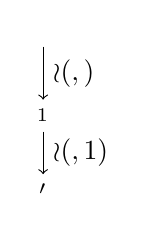
\begin{tikzpicture}[
    state/.style={},
    xscale=1,yscale=-1
]
    \node[state]	at (0,0)	(q1) {$\channelstate$};
    \node[state]	at (0,1)	(h1) {$\hstate_1$};
    \node[state]	at (0,2)	(q2) {$\channelstate'$};

    \draw[->] (q1) -- node[right] {$\wr(\xwr,\channelmessage)$} (h1);
    \draw[->] (h1) -- node[right] {$\wr(\yvar,1)$} (q2);
\end{tikzpicture}
\bigskip
\caption{send operation $\channelstate \to[!\channelmessage] \channelstate'$}
\end{subfigure}

\bigskip
\bigskip

% receive
\begin{subfigure}{\linewidth}
\centering
\begin{tikzpicture}[
    state/.style={},
    xscale=1,yscale=-1
]
    \node[state]	at (0,0)	(q1) {$\channelstate$};
    \node[state]	at (0,1)	(h1) {$\hstate_1$};
    \node[state]	at (0,2)	(h2) {$\hstate_2$};
    \node[state]	at (0,3)	(h3) {$\hstate_3$};
    \node[state]	at (0,4)	(q2) {$\channelstate'$};

    \node[state]	at (4,1)	(h4) {$\hstate_4$};
    \node[state]	at (4,2)	(h5) {$\hstate_5$};
    \node[state]	at (4,3)	(h6) {$\hstate_6$};

    \draw[->] (q1) -- node[right] {$\nop$} (h1);
    \draw[->] (h1) -- node[right] {$\rd(\xrd,\channelmessage)$} (h2);
    \draw[->] (h2) -- node[right] {$\rd(\xrd,\bot)$} (h3);
    \draw[->] (h3) -- node[right] {$\nop$} (q2);

    \draw[->] (h1) -- node[above] {$\mf$} (h4);
    \draw[->] (h4) -- node[right] {$\nop$} (h5);
    \draw[->] (h5) -- node[right] {$\rd(\xwr,\bot)$} (h6);
\end{tikzpicture}
\bigskip
\caption{receive operation $\channelstate \to[?\channelmessage] \channelstate'$}
\end{subfigure}

\caption{$\process^1$ of the A-TSO reduction from PCS}
\label{fig:a-reduction-1}
\end{figure}
